
\documentclass[a4paper,12pt]{article}
%%%%%%%%%%%%%%%%%%%%%%%%%%%%%%%%%%%%%%%%%%%%%%%%%%%%%%%%%%%%%%%%%%%%%%%%%%%%%%%%%%%%%%%%%%%%%%%%%%%%%%%%%%%%%%%%%%%%%%%%%%%%%%%%%%%%%%%%%%%%%%%%%%%%%%%%%%%%%%%%%%%%%%%%%%%%%%%%%%%%%%%%%%%%%%%%%%%%%%%%%%%%%%%%%%%%%%%%%%%%%%%%%%%%%%%%%%%%%%%%%%%%%%%%%%%%
\usepackage{eurosym}
\usepackage{vmargin}
\usepackage{amsmath}
\usepackage{graphics}
\usepackage{epsfig}
\usepackage{framed}
\usepackage{subfigure}
\usepackage{fancyhdr}
\usepackage{framed}
\usepackage{subfiles}
\usepackage{graphics}
\usepackage{newlfont}
\usepackage{eurosym}
\usepackage{amsmath,amsthm,amsfonts}
\usepackage{amsmath}
\usepackage{enumerate}
\usepackage{color}
\usepackage{multicol}
\usepackage{amssymb}
\usepackage{multicol}
\usepackage[dvipsnames]{xcolor}
\usepackage{graphicx}

\setcounter{MaxMatrixCols}{10}
%TCIDATA{OutputFilter=LATEX.DLL}
%TCIDATA{Version=5.00.0.2570}
%TCIDATA{<META NAME="SaveForMode"CONTENT="1">}
%TCIDATA{LastRevised=Wednesday, February 23, 201113:24:34}
%TCIDATA{<META NAME="GraphicsSave" CONTENT="32">}
%TCIDATA{Language=American English}

\pagestyle{fancy}
\setmarginsrb{20mm}{0mm}{20mm}{25mm}{12mm}{11mm}{0mm}{11mm}
\lhead{MA4128} \rhead{Kevin O'Brien} \chead{Logistic Regression} %\input{tcilatex}

%http://www.electronics.dit.ie/staff/ysemenova/Opto2/CO_IntroLab.pdf
\begin{document}
	
\section{Binary Classification}	


\subsection{The Logistic Regression Equation}
The form of the logistic regression equation is:
\begin{framed}
	\[ \mbox{logit}[p(x)] =  log \left(\frac{p(x)}{1-p(x)} \right) = b_0 + b_1x_1 + b_2x_2 + b_3x_3 + \ldots \]
\end{framed}
This looks just like a linear regression and although logistic regression finds a ‘best
fitting’ equation, just as linear regression does, the principles on which it does so are
rather different. Instead of using a least-squared deviations criterion for the best fit, it
uses a maximum likelihood method, which maximizes the probability of getting the
observed results given the fitted regression coefficients. A consequence of this is that the
goodness of fit and overall significance statistics used in logistic regression are different
from those used in linear regression.

The probability that a case is in a particular category,p, can be calculated with the following formula (which is simply another rearrangement of the previous formula).

\[p = \frac{exp(b_0 + b_1x_1 + b_2x_2 + b_3x_3 + \ldots)}{1 + exp(b_0 + b_1x_1 + b_2x_2 + b_3x_3 + \ldots)}\]

\newpage



\subsection{Category Prediction Table}

\begin{itemize}
	\item It is very common to use binomial logistic regression to predict whether cases can be correctly classified (i.e., predicted) from the independent variables. Therefore, it becomes necessary to have a method to assess the effectiveness of the predicted classification against the actual classification.
	\item  There are many methods to assess this with their usefulness oftening depending on the nature of the study conducted. However, all methods revolve around the observed and predicted classifications, which are presented in the ``\texttt{Classification Table}", as shown below:
	
	
	\begin{figure}
		\centering
		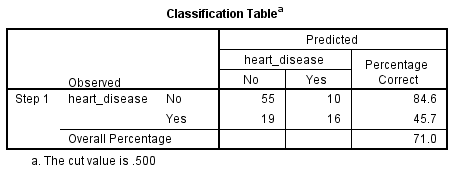
\includegraphics[width=0.8\linewidth]{images/BLogReg-Table}
	\end{figure}
	
	
	
	\item Firstly, notice that the table has a subscript which states, ``\texttt{The cut value is .500}". This means that if the probability of a case being classified into the ``\textbf{\textit{yes}}" category is greater than .500, then that particular case is classified into the ``\textbf{\textit{yes}}" category. 
	Otherwise, the case is classified as in the ``\textbf{\textit{no}}" category. 
\end{itemize}




\subsection{Omnibus Test for Model Coefficients}
The overall significance is tested using what SPSS calls the \textbf{\textit{Model Chi-square}}, which is derived from the likelihood of observing the actual data under the assumption that the model that has been fitted is accurate. There are two hypotheses to test in relation to the overall fit of the model:


 \begin{itemize}
 \item[$H_0$] The model is a good fitting model.
 \item[$H_1$] The model is not a good fitting model (i.e. the predictors have a significant effect).
 \end{itemize}
 In our case model chi square has 2 degrees of freedom, a value of 24.096 and a probability of $p < 0.000$.

Thus, the indication is that the model has a poor fit, with the model containing only the constant indicating that the predictors do have a significant effect and create essentially a different model. So we need to look closely at
the predictors and from later tables determine if one or both are significant predictors.

This table has 1 step. This is because we are entering both variables and at the same
time providing only one model to compare with the constant model. In stepwise logistic regression there are a number of steps listed in the table as each variable is added or
removed, creating different models. The step is a measure of the improvement in the
predictive power of the model since the previous step. ( I will revert to this next class).

%The likelihood function can be thought of as a measure of how well a candidate model fits the data (although that is a very simplistic definition). The AIC criterion is based on the Likelihood function.
%The likelihood function of a fitted model is commonly re-expressed as -2LL (i.e. The log of the likelihood times minus 2).

%The difference between –2LL for the best-fitting model and –2LL for the null hypothesis model (in which all the b values are set to zero in block 0) is distributed like
%chi squared, with degrees of freedom equal to the number of predictors; this difference
%is the Model chi square that SPSS refers to. Very conveniently, the difference between –2LL values for models with successive terms added also has a chi squared distribution,
%so when we use a stepwise procedure, we can use chi-squared tests to find out if adding
%one or more extra predictors significantly improves the fit of our model.


\subsection{Model Summary Table}


The likelihood function can be thought of as a measure of how well a candidate model fits the data (although that is a very simplistic definition). The AIC criterion is based on the Likelihood function.
The likelihood function of a fitted model is commonly re-expressed as -2LL (i.e. The log of the likelihood times minus 2). The –2LL value from the Model Summary table below is 17.359.

Although there is no close analogous statistic in logistic regression to
the coefficient of determination $R^2$ the Model Summary Table provides some approximations. Cox and Snell’s R-Square attempts to imitate multiple R-Square based on ‘likelihood’, but its maximum can be (and usually is) less than 1.0, making it difficult to interpret. Here it is indicating that 55.2\% of the variation in the DV is explained by the
logistic model. The Nagelkerke modification that does range from 0 to 1 is a more reliable
measure of the relationship. Nagelkerke’s $R^2$ will normally be higher than the Cox and Snell measure. Nagelkerke’s $R^2$ is part of SPSS output in the ‘Model Summary’ table and is the most-reported of the R-squared estimates. In our case it is 0.737, indicating a moderately strong relationship of 73.7\% between the predictors and the prediction.
\newpage
\subsection{Hosmer and Lemeshow  Statistic}
An alternative to model chi square is the Hosmer and Lemeshow test
which divides subjects into 10 ordered groups of subjects and then compares the number
actually in the each group (observed) to the number predicted by the logistic regression
model (predicted). The 10 ordered groups are created based on their estimated probability; those with estimated probability below .1 form one group, and so on, up to those with probability .9 to 1.0.

Each of these categories is further divided into two groups based on the actual observed outcome variable (success, failure). The expected frequencies for each of the cells are obtained from the model. A probability (p) value is
computed from the chi-square distribution with 8 degrees of freedom to test the fit of the logistic model.

If the H-L goodness-of-fit test statistic is greater than .05, as we want for well-fitting models, we fail to reject the null hypothesis that there is no difference between observed and model-predicted values, implying that the model’s estimates fit the data at an acceptable level. That is, well-fitting models show non-significance on the
H-L goodness-of-fit test. This desirable outcome of non-significance indicates that the
model prediction does not significantly differ from the observed.

The H-L statistic assumes sampling adequacy, with a rule of thumb being enough cases so that 95\% of cells (typically, 10 decile groups times 2 outcome categories = 20 cells) have an expected frequency $>$ 5. Our H-L statistic has a significance of .605 which means that it is not statistically significant and therefore our model is quite a
good fit.
\begin{figure}[h!]
\begin{center}
  % Requires \usepackage{graphicx}
  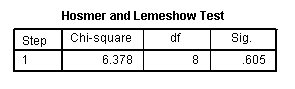
\includegraphics[scale=0.6]{images/Logistic7A}\\
  \caption{Hosmer and Lemeshow Statistic}
\end{center}
\end{figure}

\begin{figure}[h!]
\begin{center}
  % Requires \usepackage{graphicx}
  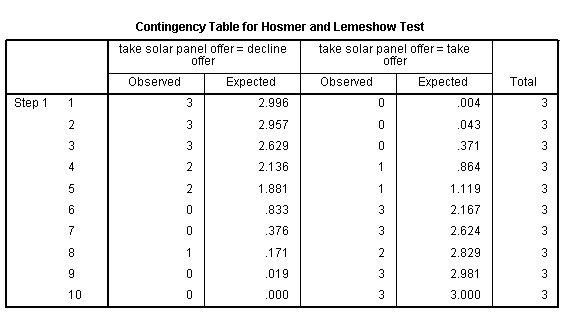
\includegraphics[scale=0.6]{images/Logistic6}\\
  \caption{Hosmer and Lemeshow Table}
\end{center}
\end{figure}
\newpage
\subsection{Classification Table}
Rather than using a goodness-of-fit statistic, we often want to look at the proportion of cases we have managed to classify correctly. For this we need to look at the classification table printed out by SPSS, which tells us how many of the cases where the observed values of the dependent variable were 1 or 0 respectively have
been correctly predicted.

In the Classification table, the columns are the two predicted values of the dependent, while the rows are the two observed (actual) values of the dependent. In a perfect model, all cases will be on the diagonal and the
overall percent correct will be 100\%. In this study, 87.5\% were correctly classified for the take offer group and 92.9\% for the decline offer group. Overall 90\% were correctly classified. This is a considerable improvement on the 53.3\% correct classification with the constant model so we know that the model with predictors is a significantly better mode.
\begin{figure}[h!]
	\begin{center}
		% Requires \usepackage{graphicx}
		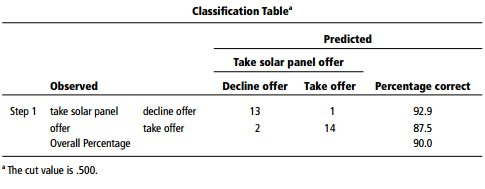
\includegraphics[scale=0.6]{images/Logistic7}\\
		\caption{Classification Table}
	\end{center}
\end{figure}

\subsection{Classification Plot} 
The classification plot or histogram of predicted probabilities
provides a visual demonstration of the correct and incorrect predictions. Also called the `\texttt{classplot}' or the `\texttt{plot of observed groups and predicted probabilities}?,it is another very useful piece of information from the SPSS output when one chooses
\texttt{Classification plots}' under the Options button in the Logistic Regression dialogue box.

\subsection{Interpreting the Classifcation Table}
Whilst the classification table appears to be very simple, it actually provides a lot of important information about your binomial logistic regression result, including:


\begin{itemize}
	\item[A.] The \textbf{percentage accuracy in classification (PAC)}, which reflects the percentage of cases that can be correctly classified as "no" heart disease with the independent variables added (not just the overall model).
	\item[B.] \textbf{Sensitivity}, which is the percentage of cases that had the observed characteristic (e.g., "yes" for heart disease) which were correctly predicted by the model (i.e., true positives).
	\item[C.] \textbf{Specificity}, which is the percentage of cases that did not have the observed characteristic (e.g., "no" for heart disease) and were also correctly predicted as not having the observed characteristic (i.e., true negatives).
	\item[D.] The \textbf{positive predictive value}, which is the percentage of correctly predicted cases "with" the observed characteristic compared to the total number of cases predicted as having the characteristic.
	\item[E.] The \textbf{negative predictive value}, which is the percentage of correctly predicted cases ``without" the observed characteristic compared to the total number of cases predicted as not having the characteristic.
\end{itemize}
%--------------------------------------------------------------------------------------%




	
\subsection{SPSS Output}
The variable Vote2005 is a binary variable describing turnout at a general election. The predictor variables are gender and age.
\begin{center}
	\begin{figure}[h!]
		% Requires \usepackage{graphicx}
		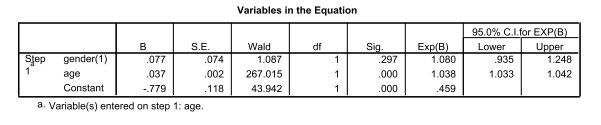
\includegraphics[scale=0.6]{images/LogWeek10B.jpg}\\
		\caption{General Election 2005}
	\end{figure}
\end{center}

% Image LogWeek10-B

\[\mbox{logit(vote2005)} = -.779 + .077\mbox{gender(1)}+.037\mbox{age}\]

The age coefficient is statistically significant. Exp(B) for age is 1.038, which
means for each year different in age, the person is 1.038 times more likely to turn
out to vote, having allowed for gender in the model. Eg. a 21 year old is 1.038
times as likely to turn out to vote than a 20 year old. This might not seem much
of a difference but a 20 year difference leads to a person being $1.038^20 = 2.11$
times more likely to turn out to vote. E.g. a 40 year old is 2.11 times more likely to
turn out to vote than a 20 year old, having allowed for gender in the model.


The gender coefficient is not statistically significant.



\end{document}